% !TEX spellcheck = en_US



% ~~~~~~~~~~~~~~~~~~~~~~~~~~~~~~~~~~~~~~~ V
% (NC) 2026 Haluk Bingol
% github.com/halukbingol/LaTeX-Templates
%
% Licensees may copy, distribute, display, and perform the work and make derivative works 
% and remixes based on it only for non-commercial purposes. 
% ~~~~~~~~~~~~~~~~~~~~~~~~~~~~~~~~~~~~~~~ A




% =====================================================================
%  Unit Testing with JUnit -- Senior Level: the Platform, Migration, Suites, Properties and Test Strategy
%  ---------------------------------------------------------------------
%  Built on hblib/Template/hblibTemplate.tex with the libraries in ../../hblib/.
%  Programs and their real outputs are in codeoutput/:
%     codeoutput/<Name>.java  a program (classes without main() are only compiled)
%     codeoutput/<Name>.sh    a terminal session, run in a copy of codeoutput/<Name>/
%     codeoutput/<Name>.txt   what it printed, made by:  bash run_examples.sh
% =====================================================================

\documentclass[aspectratio=169,10pt,compress]{beamer}

% ~~~~~~~~~~~~~~~~~~~~~~~~~~~~~~~~~~~~~~~~~~~~~~~~~~~~~~~~~~~~~~~~~ V hblib
	\usepackage{../../hblib/hblibPresentation} % lib presentation: theme, i/N, \hSection, algorithm2e, ...
	\usepackage{../../hblib/hblibCodeoutput} % lib code + output: \lstcode, \lstterminal, ...
	\usepackage{../../hblib/hblibDatastructures} % lib data structures: \hString, \hStack, \hQueue
% ~~~~~~~~~~~~~~~~~~~~~~~~~~~~~~~~~~~~~~~~~~~~~~~~~~~~~~~~~~~~~~~~~ A hblib


% theme, i/N, fonts (T1, lmodern), booktabs, xcolor, array (L{width} columns), listings, tikz,
% algorithm2e (\small captions, \Fn) and the color gitred come from the hblib libraries




% +++++++++++++++++++++++++++++++++++++++ V specific
\DontPrintSemicolon % in algorithms
\newcommand{\win}{\textbf{Windows}}
\newcommand{\mac}{\textbf{macOS}}
% +++++++++++++++++++++++++++++++++++++++ A specific

% ---------------------------------------------------------------------
\title{Unit Testing with JUnit}
\subtitle{Senior Level: the Platform, Migration, Suites, Properties and Test Strategy}
\author[Bingol]{Haluk O. Bingol}

\institute[FCIS]{
    Faculty of Computer and Information Sciences\\
    Yeditepe University
}
\date{
	{\tiny \hbTimeStamp}
}

\begin{document}




% ~~~~~~~~~~~~~~~~~~~~~~~~~~~~~~~~~~~~~~ V frm
\begin{frame}[t,fragile]
  \titlepage
\end{frame}
% ~~~~~~~~~~~~~~~~~~~~~~~~~~~~~~~~~~~~~~ A frm




% ~~~~~~~~~~~~~~~~~~~~~~~~~~~~~~~~~~~~~~ V frm
\begin{frame}[t,fragile] \frametitle{Outline}
  \begin{columns}[T]
    \begin{column}{0.48\textwidth}
      \tableofcontents[sections={1-4}, hideallsubsections]
    \end{column}
    \begin{column}{0.48\textwidth}
      \tableofcontents[sections={5-7}, hideallsubsections]
    \end{column}
  \end{columns}
\end{frame}
% ~~~~~~~~~~~~~~~~~~~~~~~~~~~~~~~~~~~~~~ A frm

% ~~~~~~~~~~~~~~~~~~~~~~~~~~~~~~~~~~~~~~ V
\hSection[Platform]{The JUnit Platform}
% ~~~~~~~~~~~~~~~~~~~~~~~~~~~~~~~~~~~~~~ A




% ~~~~~~~~~~~~~~~~~~~~~~~~~~~~~~~~~~~~~~ V frm
\begin{frame}[t,fragile] \frametitle{One platform, many engines}
  \begin{center}
  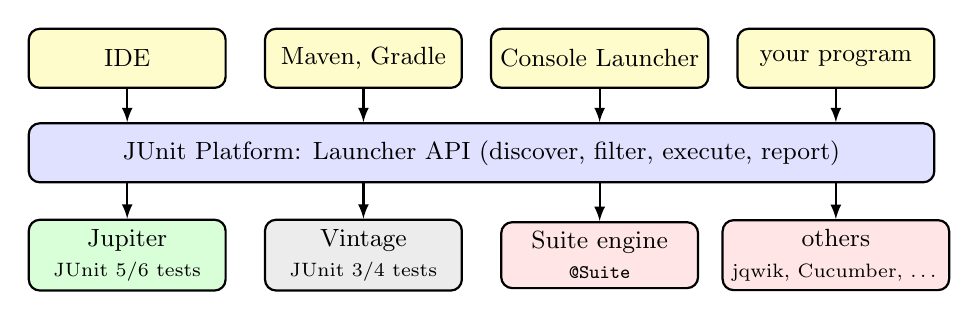
\begin{tikzpicture}[b/.style={draw, thick, rounded corners, minimum width=2.5cm, minimum height=0.75cm, font=\small, align=center}]
    \node[b, fill=yellow!20] (ide) at (-4.5,2.2) {IDE};
    \node[b, fill=yellow!20] (mvn) at (-1.5,2.2) {Maven, Gradle};
    \node[b, fill=yellow!20] (con) at (1.5,2.2)  {Console Launcher};
    \node[b, fill=yellow!20] (own) at (4.5,2.2)  {your program};
    \node[b, fill=blue!12, minimum width=11.5cm] (l) at (0,1) {JUnit Platform: Launcher API (discover, filter, execute, report)};
    \node[b, fill=green!15] (j) at (-4.5,-0.3) {Jupiter\\ \scriptsize JUnit 5/6 tests};
    \node[b, fill=gray!15]  (v) at (-1.5,-0.3) {Vintage\\ \scriptsize JUnit 3/4 tests};
    \node[b, fill=red!10]   (s) at (1.5,-0.3)  {Suite engine\\ \scriptsize \texttt{@Suite}};
    \node[b, fill=red!10]   (o) at (4.5,-0.3)  {others\\ \scriptsize jqwik, Cucumber, \dots};
    \foreach \x in {ide, mvn, con, own} \draw[-latex, thick] (\x) -- (\x |- l.north);
    \foreach \x in {j, v, s, o} \draw[-latex, thick] (\x |- l.south) -- (\x);
  \end{tikzpicture}
  \end{center}
  \begin{itemize}\small
    \item Tools talk only to the \textbf{Launcher}; each \textbf{TestEngine} finds and runs its own kind of tests.
    \item A new test style (properties, BDD scenarios) is a new engine: no tool needs to change.
  \end{itemize}
\end{frame}
% ~~~~~~~~~~~~~~~~~~~~~~~~~~~~~~~~~~~~~~ A frm




% ~~~~~~~~~~~~~~~~~~~~~~~~~~~~~~~~~~~~~~ V frm
\begin{frame}[t,fragile] \frametitle{Running tests from your own program}
  \begin{columns}[T]
    \begin{column}{0.49\textwidth}
      \lstcode[basicstyle=\ttfamily\tiny, lastline=16]{codeoutput/Launcher/MyRunner.java}{Java}
    \end{column}
    \begin{column}{0.49\textwidth}
      \lstcode[basicstyle=\ttfamily\tiny, firstline=17, firstnumber=17]{codeoutput/Launcher/MyRunner.java}{Java}
    \end{column}
  \end{columns}
\end{frame}
% ~~~~~~~~~~~~~~~~~~~~~~~~~~~~~~~~~~~~~~ A frm




% ~~~~~~~~~~~~~~~~~~~~~~~~~~~~~~~~~~~~~~ V frm
\begin{frame}[t,fragile] \frametitle{The Launcher API at work}
  \begin{columns}[T]
    \begin{column}{0.5\textwidth}
      \lstterminal[basicstyle=\ttfamily\tiny]{codeoutput/Launcher.txt}
    \end{column}
    \begin{column}{0.46\textwidth}
      \begin{itemize}\small
        \item Build a \texttt{LauncherDiscoveryRequest} with selectors (class, package, method, class path\dots) and filters.
        \item Listeners receive every event: that is how IDEs draw their tree and how build tools write XML reports.
        \item Here: our own one-line-per-test report and a summary.
      \end{itemize}
    \end{column}
  \end{columns}
\end{frame}
% ~~~~~~~~~~~~~~~~~~~~~~~~~~~~~~~~~~~~~~ A frm

% ~~~~~~~~~~~~~~~~~~~~~~~~~~~~~~~~~~~~~~ V
\hSection[Migration]{From JUnit 4 to JUnit 6}
% ~~~~~~~~~~~~~~~~~~~~~~~~~~~~~~~~~~~~~~ A




% ~~~~~~~~~~~~~~~~~~~~~~~~~~~~~~~~~~~~~~ V frm
\begin{frame}[t,fragile] \frametitle{The same test, two generations}
  \begin{columns}[T]
    \begin{column}{0.48\textwidth}
      \lstcode[basicstyle=\ttfamily\tiny]{codeoutput/Vintage/LegacyAccountTest.java}{Java}
    \end{column}
    \begin{column}{0.5\textwidth}
      \lstcode[basicstyle=\ttfamily\tiny]{codeoutput/Vintage/AccountDepositsTest.java}{Java}
    \end{column}
  \end{columns}
\end{frame}
% ~~~~~~~~~~~~~~~~~~~~~~~~~~~~~~~~~~~~~~ A frm




% ~~~~~~~~~~~~~~~~~~~~~~~~~~~~~~~~~~~~~~ V frm
\begin{frame}[t,fragile] \frametitle{Both run side by side}
  \begin{columns}[T]
    \begin{column}{0.56\textwidth}
      \lstterminal[basicstyle=\ttfamily\tiny]{codeoutput/Vintage.txt}
    \end{column}
    \begin{column}{0.40\textwidth}
      \begin{itemize}\small
        \item The \textbf{Vintage} engine runs JUnit 4 tests on the platform: migrate one class at a time.
        \item \texttt{--scan-classpath}: find every test class in \texttt{bin}.
        \item JUnit 6 \textbf{deprecates} Vintage: plan the migration, do not stay on it.
      \end{itemize}
    \end{column}
  \end{columns}
\end{frame}
% ~~~~~~~~~~~~~~~~~~~~~~~~~~~~~~~~~~~~~~ A frm




% ~~~~~~~~~~~~~~~~~~~~~~~~~~~~~~~~~~~~~~ V frm
\begin{frame}[t,fragile] \frametitle{Migration table}
  \begin{center}\footnotesize
  \begin{tabular}{@{}ll@{}}
    \toprule
    \textbf{JUnit 4}                                  & \textbf{JUnit Jupiter (5 and 6)} \\
    \midrule
    \texttt{org.junit.Test}, \texttt{public} methods  & \texttt{org.junit.jupiter.api.Test}, package-private is enough \\
    \texttt{@Before}, \texttt{@After}                 & \texttt{@BeforeEach}, \texttt{@AfterEach} \\
    \texttt{@BeforeClass}, \texttt{@AfterClass}       & \texttt{@BeforeAll}, \texttt{@AfterAll} \\
    \texttt{@Ignore}                                  & \texttt{@Disabled} \\
    \texttt{@Test(expected = X.class)}                & \texttt{assertThrows(X.class, \dots)} \\
    \texttt{assertEquals("msg", e, a)}                & \texttt{assertEquals(e, a, "msg")}: the message is \textbf{last} \\
    \texttt{@RunWith}, \texttt{@Rule}                 & \texttt{@ExtendWith}, extensions \\
    \texttt{@Category}                                & \texttt{@Tag} \\
    \bottomrule
  \end{tabular}
  \end{center}
  \small Tools such as OpenRewrite automate most of this table. \hRemark{Not run here}.
\end{frame}
% ~~~~~~~~~~~~~~~~~~~~~~~~~~~~~~~~~~~~~~ A frm




% ~~~~~~~~~~~~~~~~~~~~~~~~~~~~~~~~~~~~~~ V frm
\begin{frame}[t,fragile] \frametitle{What changed in JUnit 6 (September 2025)}
  \begin{columns}[T]
    \begin{column}{0.5\textwidth}
      \begin{itemize}\small
        \item \textbf{Java 17} is the minimum.
        \item \textbf{One version number} for Platform, Jupiter and Vintage (6.0.0; before: Platform 1.x, Jupiter 5.x).
        \item The Console Launcher needs a command: \texttt{execute}, \texttt{discover}, \texttt{engines}.
        \item Vintage engine and \texttt{junit-jupiter-migrationsupport} \textbf{deprecated}; the JUnit 4 runner
              \texttt{JUnitPlatform} removed.
      \end{itemize}
    \end{column}
    \begin{column}{0.46\textwidth}
      \begin{itemize}\small
        \item JSpecify null annotations on the whole API.
        \item \texttt{@CsvSource} parsed by FastCSV; Kotlin \texttt{suspend} test methods.
        \item 6.1 (May 2026): \texttt{@DefaultLocale}, \texttt{@DefaultTimeZone}, a new parallel executor.
        \item Current: \textbf{6.1.3}. The examples here run on Jupiter 5.10/Platform 1.9; the API they use is unchanged.
      \end{itemize}
    \end{column}
  \end{columns}
\end{frame}
% ~~~~~~~~~~~~~~~~~~~~~~~~~~~~~~~~~~~~~~ A frm

% ~~~~~~~~~~~~~~~~~~~~~~~~~~~~~~~~~~~~~~ V
\hSection[Suites]{Suites}
% ~~~~~~~~~~~~~~~~~~~~~~~~~~~~~~~~~~~~~~ A




% ~~~~~~~~~~~~~~~~~~~~~~~~~~~~~~~~~~~~~~ V frm
\begin{frame}[t,fragile] \frametitle{A suite: tests chosen by rules}
  \begin{columns}[T]
    \begin{column}{0.5\textwidth}
      \lstcode[basicstyle=\ttfamily\tiny, firstline=6, firstnumber=6]{codeoutput/Suite/FastSuite.java}{Java}
      \lstcode[basicstyle=\ttfamily\tiny, firstline=8, firstnumber=8]{codeoutput/Suite/grades/LetterTest.java}{Java}
    \end{column}
    \begin{column}{0.48\textwidth}
      \uncover<2->{\lstterminal[basicstyle=\ttfamily\tiny]{codeoutput/Suite.txt}}
      \begin{itemize}\small
        \item The suite engine runs whatever matches: every \texttt{fast} test in package \texttt{grades}; new classes join automatically.
      \end{itemize}
    \end{column}
  \end{columns}
\end{frame}
% ~~~~~~~~~~~~~~~~~~~~~~~~~~~~~~~~~~~~~~ A frm

% ~~~~~~~~~~~~~~~~~~~~~~~~~~~~~~~~~~~~~~ V
\hSection[Properties]{Property-Based Testing}
% ~~~~~~~~~~~~~~~~~~~~~~~~~~~~~~~~~~~~~~ A




% ~~~~~~~~~~~~~~~~~~~~~~~~~~~~~~~~~~~~~~ V frm
\begin{frame}[t,fragile] \frametitle{Examples versus properties}
  \begin{columns}[T]
    \begin{column}{0.4\textwidth}
      \lstcode[basicstyle=\ttfamily\tiny]{codeoutput/Property/MySort.java}{Java}
      \begin{itemize}\small
        \item Example tests: ``\texttt{[3, 1, 2]} becomes \texttt{[1, 2, 3]}''.
        \item A \textbf{property}: for \emph{every} array, \texttt{MySort} agrees with \texttt{Arrays.sort}.
      \end{itemize}
    \end{column}
    \begin{column}{0.58\textwidth}
      \lstcode[basicstyle=\ttfamily\tiny]{codeoutput/Property/SortPropertyTest.java}{Java}
    \end{column}
  \end{columns}
\end{frame}
% ~~~~~~~~~~~~~~~~~~~~~~~~~~~~~~~~~~~~~~ A frm




% ~~~~~~~~~~~~~~~~~~~~~~~~~~~~~~~~~~~~~~ V frm
\begin{frame}[t,fragile] \frametitle{200 random arrays find the bug}
  \begin{columns}[T]
    \begin{column}{0.58\textwidth}
      \lstterminal[basicstyle=\ttfamily\tiny]{codeoutput/Property.txt}
    \end{column}
    \begin{column}{0.38\textwidth}
      \begin{itemize}\small
        \item A fixed seed (2026) makes the ``random cases repeatable: the same arrays on every run.
        \item Every failure starts with the first element out of place: \texttt{j > 0} should be \texttt{j >= 0}.
        \item Libraries (jqwik, an engine of its own) also \textbf{shrink} a failing case to the smallest one.
      \end{itemize}
    \end{column}
  \end{columns}
\end{frame}
% ~~~~~~~~~~~~~~~~~~~~~~~~~~~~~~~~~~~~~~ A frm

% ~~~~~~~~~~~~~~~~~~~~~~~~~~~~~~~~~~~~~~ V
\hSection[Strategy]{Test Strategy}
% ~~~~~~~~~~~~~~~~~~~~~~~~~~~~~~~~~~~~~~ A




% ~~~~~~~~~~~~~~~~~~~~~~~~~~~~~~~~~~~~~~ V frm
\begin{frame}[t,fragile] \frametitle{The test pyramid}
  \begin{columns}[T]
    \begin{column}{0.48\textwidth}
      \begin{center}
      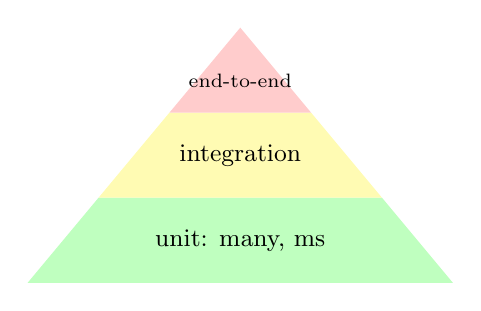
\begin{tikzpicture}[scale=0.9]
        \fill[green!25] (-3,0) -- (3,0) -- (2,1.2) -- (-2,1.2) -- cycle;
        \fill[yellow!30] (-2,1.2) -- (2,1.2) -- (1,2.4) -- (-1,2.4) -- cycle;
        \fill[red!20] (-1,2.4) -- (1,2.4) -- (0,3.6) -- cycle;
        \node[font=\small] at (0,0.6) {unit: many, ms};
        \node[font=\small] at (0,1.8) {integration};
        \node[font=\scriptsize] at (0,2.85) {end-to-end};
      \end{tikzpicture}
      \end{center}
    \end{column}
    \begin{column}{0.48\textwidth}
      \begin{itemize}\small
        \item \textbf{Unit}: one class, no I/O; thousands, run on every save.
        \item \textbf{Integration}: real database, files, HTTP (e.g.\ Testcontainers starts a database in Docker); slower, fewer.
        \item \textbf{End-to-end}: the whole system through its UI or API; few, slow, brittle.
        \item All can be JUnit tests; tags and suites decide what runs where.
      \end{itemize}
    \end{column}
  \end{columns}
\end{frame}
% ~~~~~~~~~~~~~~~~~~~~~~~~~~~~~~~~~~~~~~ A frm




% ~~~~~~~~~~~~~~~~~~~~~~~~~~~~~~~~~~~~~~ V frm
\begin{frame}[t,fragile] \frametitle{Keeping a large test suite healthy}
  \begin{columns}[T]
    \begin{column}{0.48\textwidth}
      \begin{block}{Flaky tests}
        \small A test that sometimes fails without a code change: time, order, parallelism, network.
        Quarantine it (\texttt{@Tag("flaky")}), fix the cause, never just re-run until green.
      \end{block}
      \begin{block}{Speed}
        \small Parallel execution, test selection by changed modules, slow tests nightly.
      \end{block}
    \end{column}
    \begin{column}{0.48\textwidth}
      \begin{block}{Quality of the tests}
        \small Coverage finds gaps; mutation testing (PIT) checks that tests fail when the code is wrong;
        review test code like production code.
      \end{block}
      \begin{block}{Test data}
        \small Synthetic data only: no real student names, ID numbers or grades in test files or fixtures
        (KVKK, the Turkish personal data law; GDPR in the EU).
      \end{block}
    \end{column}
  \end{columns}
\end{frame}
% ~~~~~~~~~~~~~~~~~~~~~~~~~~~~~~~~~~~~~~ A frm

% ~~~~~~~~~~~~~~~~~~~~~~~~~~~~~~~~~~~~~~ V
\hSection[Summary]{Summary}
% ~~~~~~~~~~~~~~~~~~~~~~~~~~~~~~~~~~~~~~ A




% ~~~~~~~~~~~~~~~~~~~~~~~~~~~~~~~~~~~~~~ V frm
\begin{frame}[t,fragile] \frametitle{Big ideas}
  \begin{itemize}
    \item The JUnit Platform separates \textbf{tools} (IDE, Maven, Gradle, console) from \textbf{engines} (Jupiter, Vintage, Suite, \dots).
    \item The Launcher API and listeners let any program discover, run and report tests.
    \item JUnit 4 tests run under Vintage during a migration; JUnit 6 deprecates it and requires Java 17.
    \item Suites select tests by package, tag or name; tags separate fast from slow.
    \item Properties with many generated inputs find bugs that hand-picked examples miss.
    \item A healthy suite is a pyramid: many fast unit tests, few slow end-to-end tests, no flaky ones, no real personal data.
  \end{itemize}
\end{frame}
% ~~~~~~~~~~~~~~~~~~~~~~~~~~~~~~~~~~~~~~ A frm




% ~~~~~~~~~~~~~~~~~~~~~~~~~~~~~~~~~~~~~~ V frm
\begin{frame}[t,fragile] \frametitle{Projects}
  \begin{enumerate}\small
    \item \textbf{A test report}: extend \texttt{MyRunner} into a listener that writes a Markdown report with the slowest 10 tests.
    \item \textbf{Migration}: take an old JUnit 4 project from GitHub, run it under Vintage, migrate it class by class to JUnit 6.
    \item \textbf{Properties}: write property tests for a \texttt{TcKimlik} generator: every generated number must be valid.
    \item \textbf{Mutation testing}: run PIT on a project of yours, kill the surviving mutants with better assertions.
    \item \textbf{Integration}: test a small JDBC repository against a real PostgreSQL started by Testcontainers.
  \end{enumerate}
\end{frame}
% ~~~~~~~~~~~~~~~~~~~~~~~~~~~~~~~~~~~~~~ A frm




% ~~~~~~~~~~~~~~~~~~~~~~~~~~~~~~~~~~~~~~ V frm
\begin{frame}[t,fragile]
	\begin{center}
		\vspace{4cm}
		\hRemark{\Huge Questions?}
	\end{center}
\end{frame}
% ~~~~~~~~~~~~~~~~~~~~~~~~~~~~~~~~~~~~~~ A frm



\end{document}
